\documentclass{beamer}
\usepackage[utf8]{inputenc}

\usetheme{Madrid}
\usecolortheme{default}
\usepackage{amsmath,amssymb,amsfonts,amsthm}
\usepackage{txfonts}
\usepackage{tkz-euclide}
\usepackage{listings}
\usepackage{adjustbox}
\usepackage{array}
\usepackage{tabularx}
\usepackage{gvv}
\usepackage{lmodern}
\usepackage{circuitikz}
\usepackage{tikz}
\usepackage{graphicx}

\setbeamertemplate{page number in head/foot}[totalframenumber]

\usepackage{tcolorbox}
\tcbuselibrary{minted,breakable,xparse,skins}



\definecolor{bg}{gray}{0.95}
\DeclareTCBListing{mintedbox}{O{}m!O{}}{%
  breakable=true,
  listing engine=minted,
  listing only,
  minted language=#2,
  minted style=default,
  minted options={%
    linenos,
    gobble=0,
    breaklines=true,
    breakafter=,,
    fontsize=\small,
    numbersep=8pt,
    #1},
  boxsep=0pt,
  left skip=0pt,
  right skip=0pt,
  left=25pt,
  right=0pt,
  top=3pt,
  bottom=3pt,
  arc=5pt,
  leftrule=0pt,
  rightrule=0pt,
  bottomrule=2pt,
  toprule=2pt,
  colback=bg,
  colframe=orange!70,
  enhanced,
  overlay={%
    \begin{tcbclipinterior}
    \fill[orange!20!white] (frame.south west) rectangle ([xshift=20pt]frame.north west);
    \end{tcbclipinterior}},
  #3,
}
\lstset{
    language=C,
    basicstyle=\ttfamily\small,
    keywordstyle=\color{blue},
    stringstyle=\color{orange},
    commentstyle=\color{green!60!black},
    numbers=left,
    numberstyle=\tiny\color{gray},
    breaklines=true,
    showstringspaces=false,
}
%------------------------------------------------------------

\title
{4.3.9}
\date{September 3,2025}
\author 
{AI25BTECH11003 - Bhavesh Gaikwad}



\begin{document}


\frame{\titlepage}
\begin{frame}{Question}
\centering
The vector equation of the line $\dfrac{x-5}{3} = \dfrac{y+4}{7} = \dfrac{z-6}{2}$ is?
\end{frame}


\begin{frame}[fragile]
    \frametitle{Theoretical Solution}
    Given: 
\begin{equation}
\dfrac{x-5}{3} = \dfrac{y+4}{7} = \dfrac{z-6}{2}
\end{equation}
Let $\vec{A}$ be the parallel vector of the given line.\\
Let $\vec{B}$ be the position vector of a point on the given line.\\

From Equation 1,
\begin{equation}
    \vec{A} = \myvec{3 \\ 7 \\ 2}
\end{equation}
Putting x=8 in Equation 1 to get an arbitrary point on the line,
\begin{equation}
\dfrac{8-5}{3} = \dfrac{y+4}{7} = \dfrac{z-6}{2}
\quad \Rightarrow x=8, \, y = 3, \, z=8.
\end{equation}

\begin{equation}
    \therefore \, \vec{B} = \myvec{8 \\ 3 \\ 8}
\end{equation}

\end{frame}

\begin{frame}[fragile]
\frametitle{Theoretical Solution}
From Equations 1 and 4,\\
The Vector Equation of the given line is: 
\begin{equation}
\vec{L} = \vec{B} + k\vec{A}    
\text{, Where } k \text{ is a real parameter OR } k \, \epsilon \, \mathbb{R}
\end{equation}


\begin{equation}
\boxed{\vec{L} =\myvec{8 \\ 3 \\ 8} +  k\myvec{3 \\ 7 \\ 2}}
\end{equation}
\end{frame}


\begin{frame}[fragile]
    \frametitle{Python Code}
    \begin{lstlisting}
import numpy as np
import matplotlib.pyplot as plt
from mpl_toolkits.mplot3d import Axes3D

# Direction vector A and point B
A = np.array([3, 7, 2])
B = np.array([8, 3, 8])

# Parameter k for the line
k = np.linspace(-10, 10, 400)

# Compute line points: L = B + kA
line_points = B.reshape(3,1) + np.outer(A, k)

# Create a perpendicular offset so vector A doesn't overlap the line
    \end{lstlisting}
\end{frame}

\begin{frame}[fragile]
    \frametitle{Python Code}
    \begin{lstlisting}
      # Find a vector perpendicular to A by crossing with an arbitrary vector
arbitrary = np.array([1, 0, 0])
if np.allclose(np.cross(A, arbitrary), 0):
    arbitrary = np.array([0, 1, 0])
offset_dir = np.cross(A, arbitrary)
offset_dir = offset_dir / np.linalg.norm(offset_dir)
offset = offset_dir * 2  # magnitude of offset for visibility

# Base point for drawing A offset from the line
base_point = B + offset
arrow_end = base_point + A

# Plot setup
fig = plt.figure(figsize=(8, 6))
ax = fig.add_subplot(111, projection='3d')
    \end{lstlisting}
\end{frame}

\begin{frame}[fragile]
    \frametitle{Python Code}
    \begin{lstlisting}
# Plot the line L
ax.plot(line_points[0], line_points[1], line_points[2], color='blue', label='Line L')

# Mark point B on the line
ax.scatter(B[0], B[1], B[2], color='red', s=50, label='Point B (8,3,8)')

# Draw vector A at the offset base_point
ax.quiver(base_point[0], base_point[1], base_point[2],
          A[0], A[1], A[2], color='green', length=5, normalize=False, label='Vector A')
    \end{lstlisting}
\end{frame}

\begin{frame}[fragile]
    \frametitle{Python Code}
    \begin{lstlisting}
# Labels and legend
ax.set_xlabel('X')
ax.set_ylabel('Y')
ax.set_zlabel('Z')
ax.set_title('Line L and Parallel Vector A with Point B')
ax.legend()

# Save the figure
plt.savefig('fig1.png')
plt.close()
    \end{lstlisting}
\end{frame}

\begin{frame}{Line}
   \centering
    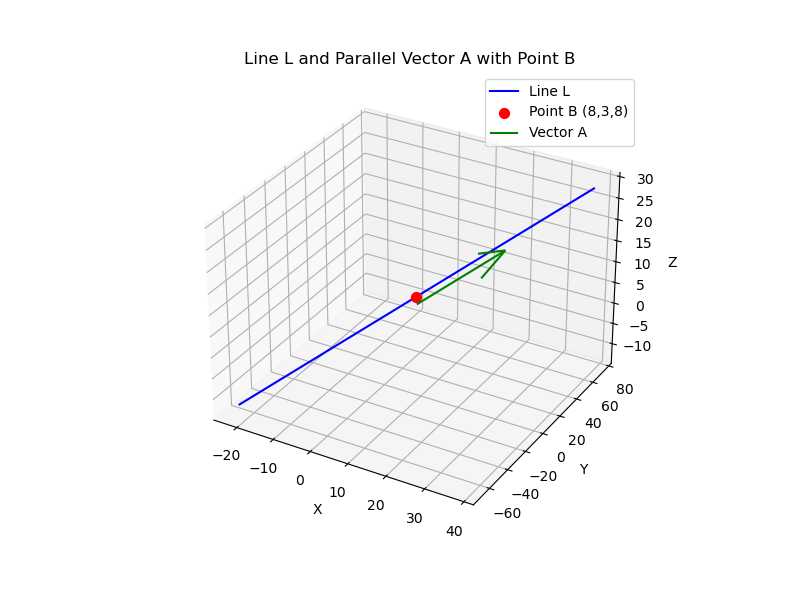
\includegraphics[width=\columnwidth, height=0.8\textheight, keepaspectratio]{figs/fig1.png}
    \label{fig:Beamer/figs/fig1.png}
\end{frame}


\end{document}